\section{Model Description}\label{sec:model_description}
The following section contains the description for all models required for the comparison done in this investigation. First, the functional unit used as a comparison point will be discussed in subsection~\ref{subsec:functional_unit}. After, thorough descriptions for the required models for both scenarios are discussed in subsections~\ref{subsec:inventory}.


\subsection{Functional Unit}\label{subsec:functional_unit}
As a first step, the topic of the functional unit must be discussed. This is a crucial step in the LCA for any product, since its very definition can sway results in a particular way. Therefore, this process was conducted with a large attention to detail in order to provide a neutral comparison between both note-taking approaches. Questions such as \textit{what?}, \textit{how much?}, \textit{how well?}, \textit{where?} and \textit{for how long?} are of special interest, leading to the following functional unit.

\renewcommand{\arraystretch}{1.5}
\begin{table}[H]
    \centering
    \begin{tabular}{M{0.4\textwidth}|M{0.5\textwidth}}
        Question & Function \\
        \hline
        \hline
        \textit{What} should the note-taking approach do?            &   Serve for note-taking for university studies with multi-color abilities\\
        \hline
        \textit{How many} materials should the approach use?         &   Enough to provide enough note-taking space for all courses\\
        \hline
        \textit{How well} should the notes be taken?                 &   Approach should deliver, readable, organized notes\\
        \hline
        \textit{Where} are the notes taken?                          &   At KU Leuven, campus Arenberg\\
        \hline
        \textit{For how long} should the approach last?              &   5 years (bachelor's + master's)
    \end{tabular}
    \caption{Functional unit for comparison between note-taking scenarios.}
    \label{tab:functional_unit}
\end{table}
\renewcommand{\arraystretch}{1}

\subsection{Test Case Inventory}\label{subsec:inventory}
Before discussing the effects for each scenario, an inventory for their unit processes must be done. This inventory contains the raw materials involved in the manufacturing process for all components used in the scenario, all processes required for the assembly as well as the transportation involved in the delivery of all physical products. It is worth noting that the materials listed in the following are not an extensive list since the use of the \textsc{SimaPro} software accounts for many often overlooked materials.

Figures~\ref{fig:inventory_pen_paper} and~\ref{fig:inventory_ipad} depict a rough representation of the inventory carried out within the \textsc{SimaPro} software for all materials and processes involved in the analog and digital note-taking scenarios, respectively. From these figures, it becomes evident that a large array of raw materials as well as energy intensive processes are required for the manufacturing (and use in the case of the digital scenario) for both scenarios. 

\begin{figure}[H]
    \centering
\begin{tikzpicture}[every text node part/.style={align=center}]
    \node(raw_mat1)[unit]{\footnotesize{Bark, Fibers,}\\\footnotesize{Cotton, etc.}};
    \node(raw_mat2)[unit, right of=raw_mat1, xshift=0.11\textwidth]{\footnotesize{Aluminum}};
    \node(raw_mat3)[unit, right of=raw_mat2, xshift=0.11\textwidth]{\footnotesize{Polystyrene}};
    \node(raw_mat4)[unit, right of=raw_mat3, xshift=0.11\textwidth]{\footnotesize{Polypropylene}};
    \node(raw_mat5)[unit, right of=raw_mat4, xshift=0.11\textwidth]{\footnotesize{Ink, solvents}};
    \node(dots1)[blank, right of=raw_mat5, xshift=0.05\textwidth]{\footnotesize{\dots}};
    
    \node(process1)[unit, below of=raw_mat1, yshift=-0.4cm]{\footnotesize{Pulping, pressing,}\\\footnotesize{calendering}};
    \node(process2)[unit, below of=raw_mat2, yshift=-0.4cm]{\footnotesize{Wire drawing}};
    \node(process3)[unit, below of=raw_mat3, yshift=-0.4cm]{\footnotesize{Injection}\\\footnotesize{moulding}};
    \node(process4)[unit, below of=raw_mat4, yshift=-0.4cm]{\footnotesize{Injection}\\\footnotesize{moulding}};
    \node(process5)[unit, below of=raw_mat5, yshift=-0.4cm]{\footnotesize{Chemical mixing}};
    \node(dots2)[blank, below of=dots1, yshift=-0.4cm]{\footnotesize{\dots}};

    \node(blank1)[blank, below of=process1, yshift=-0.4cm]{};
    \node(blank2)[blank, below of=process2, yshift=-0.4cm]{};
    \node(blank3)[blank, below of=process3, yshift=-0.4cm]{};
    \node(blank4)[blank, below of=process4, yshift=-0.4cm]{};
    \node(blank5)[blank, below of=process5, yshift=-0.4cm]{};
    \node(blank_dots)[blank, below of=dots2, yshift=-0.4cm]{};

    \node(blank_assembly)[blank, below of=blank1, yshift=-0.4cm]{};
    \node(assembly_transport)[unit, right of=blank_assembly, xshift=0.05\textwidth]{\small{Assembly}\\ \small{and}\\\small{Transportation}};
    \node(product)[unit, right of=assembly_transport, xshift=0.2\textwidth]{\small{5 Years University Studies:}\\\small{Oxford Notebooks}\\\small{BIC Ball-point pens}};
    \node(waste)[unit, below of=product, yshift=-1cm]{\small{Recycling}\\\small{Disassembly}\\\small{Landfill}};

    \draw[thick, ->, >=latex](raw_mat1.south) -- (process1.north);
    \draw[thick, ->, >=latex](raw_mat2.south) -- (process2.north);
    \draw[thick, ->, >=latex](raw_mat3.south) -- (process3.north);
    \draw[thick, ->, >=latex](raw_mat4.south) -- (process4.north);
    \draw[thick, ->, >=latex](raw_mat5.south) -- (process5.north);

    \draw[thick](process1.south) -- (blank_assembly.center);
    \draw[thick](process2.south) -- (blank2.center);
    \draw[thick](process3.south) -- (blank3.center);
    \draw[thick](process4.south) -- (blank4.center);
    \draw[thick](process5.south) -- (blank5.center);
    \draw[thick](blank_dots.center) -- (blank1.center);

    \draw[thick, ->, >=latex](blank_assembly.center) -- (assembly_transport.west);

    \draw[thick, ->, >=latex](assembly_transport.east) -- (product.west);
    \draw[thick, ->, >=latex](product.south) -- (waste.north);
    

\end{tikzpicture}
\caption{Inventory for analog note-taking scenario.}\label{fig:inventory_pen_paper}
\end{figure}

\begin{figure}[H]
    \centering
\begin{tikzpicture}[every text node part/.style={align=center}]
    \node(raw_mat1)[unit]{\footnotesize{Aluminum}};
    \node(raw_mat2)[unit, right of=raw_mat1, xshift=0.11\textwidth]{\footnotesize{Copper, Gold}};
    \node(raw_mat3)[unit, right of=raw_mat2, xshift=0.11\textwidth]{\footnotesize{Polypropylene}};
    \node(raw_mat4)[unit, right of=raw_mat3, xshift=0.11\textwidth]{\footnotesize{Polystyrene}};
    \node(raw_mat5)[unit, right of=raw_mat4, xshift=0.11\textwidth]{\footnotesize{Tin}};
    \node(dots1)[blank, right of=raw_mat5, xshift=0.05\textwidth]
    {\footnotesize{\dots}};
    
    \node(process1)[unit, below of=raw_mat1, yshift=-0.4cm]{\footnotesize{Casting}};
    \node(process2)[unit, below of=raw_mat2, yshift=-0.4cm]{\footnotesize{Electroplating}};
    \node(process3)[unit, below of=raw_mat3, yshift=-0.4cm]{\footnotesize{Injection}\\\footnotesize{moulding}};
    \node(process4)[unit, below of=raw_mat4, yshift=-0.4cm]{\footnotesize{Injection}\\\footnotesize{moulding}};
    \node(process5)[unit, below of=raw_mat5, yshift=-0.4cm]{\footnotesize{Hot air leveling}};
    \node(dots2)[blank, below of=dots1, yshift=-0.4cm]{\footnotesize{\dots}};

    \node(blank1)[blank, below of=process1, yshift=-0.4cm]{};
    \node(blank2)[blank, below of=process2, yshift=-0.4cm]{};
    \node(blank3)[blank, below of=process3, yshift=-0.4cm]{};
    \node(blank4)[blank, below of=process4, yshift=-0.4cm]{};
    \node(blank5)[blank, below of=process5, yshift=-0.4cm]{};
    \node(blank_dots)[blank, below of=dots2, yshift=-0.4cm]{};

    \node(blank_assembly)[blank, below of=blank1, yshift=-0.4cm]{};
    \node(assembly_transport)[unit, right of=blank_assembly, xshift=0.05\textwidth]{\small{Assembly}\\ \small{and}\\\small{Transportation}};
    \node(product)[unit, right of=assembly_transport, xshift=0.2\textwidth]{\small{5 Years University Studies:}\\\small{Apple iPad 10th Gen}\\\small{Apple Pencil 1st Gen}};
    \node(electricity)[unit, right of=product, xshift=0.2\textwidth]{\small{Electricity}};
    \node(waste)[unit, below of=product, yshift=-1cm]{\small{Recycling}\\\small{Disassembly}\\\small{Landfill}};

    \draw[thick, ->, >=latex](raw_mat1.south) -- (process1.north);
    \draw[thick, ->, >=latex](raw_mat2.south) -- (process2.north);
    \draw[thick, ->, >=latex](raw_mat3.south) -- (process3.north);
    \draw[thick, ->, >=latex](raw_mat4.south) -- (process4.north);
    \draw[thick, ->, >=latex](raw_mat5.south) -- (process5.north);

    \draw[thick](process1.south) -- (blank_assembly.center);
    \draw[thick](process2.south) -- (blank2.center);
    \draw[thick](process3.south) -- (blank3.center);
    \draw[thick](process4.south) -- (blank4.center);
    \draw[thick](process5.south) -- (blank5.center);
    \draw[thick](blank_dots.center) -- (blank1.center);

    \draw[thick, ->, >=latex](blank_assembly.center) -- (assembly_transport.west);

    \draw[thick, ->, >=latex](assembly_transport.east) -- (product.west);
    \draw[thick, ->, >=latex](electricity.west) -- (product.east);
    \draw[thick, ->, >=latex](product.south) -- (waste.north);
    

\end{tikzpicture}
\caption{Inventory for analog note-taking scenario..}\label{fig:inventory_ipad}
\end{figure}

Moreover, a distinction must be made between the in and outflows for each element in the inventory alongside their sources or recipients. These could come from or go to the ecosphere or the technosphere, where the ecosphere represents the natural environment and the technosphere represents industrial processes. The use of the EcoInvent database alleviates this task from the students which could become very time-intensive. This is because not many processes are straightforward and usually involve multiple inputs and outputs from all sources. Additionally, in many cases multifunctionality within the process raises many issues involving the balance for the responsibility given to the elements involved in the process. This practice involves multiple assumptions and raises many issues for the credibility of the assessment. Fortunately, EcoInvent has these assumptions embedded into its database. Simplified examples for an eco- and technosphere analysis for a single process for both note-taking strategies are given in Figures~\ref{fig:eco_technosphere_analog} and~\ref{fig:eco_technosphere_digital}.

\begin{figure}[H]
    \centering
    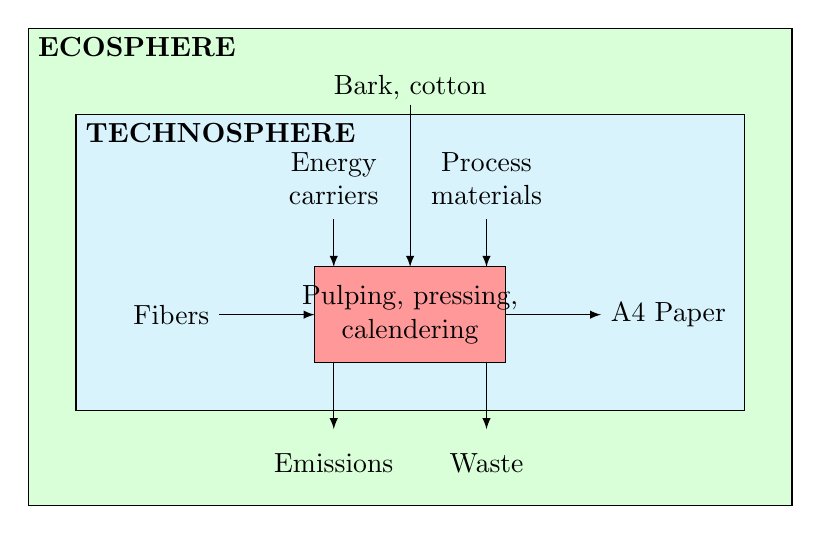
\begin{tikzpicture}[every text node part/.style={align=center}]
        \draw[fill=green!15, draw=black] (0, 0) rectangle (0.8\textwidth, 0.5\textwidth);
        \draw[fill=cyan!15, draw=black] (0.05\textwidth, 0.1\textwidth) rectangle (0.75\textwidth, 0.41\textwidth);

        \node(Ecosphere) at (0, 0.5\textwidth)[anchor=north west]{\textbf{ECOSPHERE}};
        \node(Technosphere) at (0.05\textwidth, 0.41\textwidth)[anchor=north west]{\textbf{TECHNOSPHERE}};

        \draw[fill=red!40, draw=black] (0.3\textwidth,0.15\textwidth) rectangle (0.5\textwidth,0.25\textwidth);
        \node(process) at (0.4\textwidth, 0.2\textwidth)[anchor=center]{Pulping, pressing, \\calendering};

        \draw[->, >=latex](0.4\textwidth, 0.42\textwidth) -- node[anchor=south, yshift=0.08\textwidth]{Bark, cotton}(0.4\textwidth, 0.25\textwidth);
        \draw[->, >=latex](0.2\textwidth, 0.2\textwidth) -- node[anchor=east, xshift=-0.05\textwidth]{Fibers}(0.3\textwidth, 0.2\textwidth);
        \draw[->, >=latex](0.5\textwidth, 0.2\textwidth) -- node[anchor=west, xshift=0.05\textwidth]{A4 Paper}(0.6\textwidth, 0.2\textwidth);
        \draw[->, >=latex](0.48\textwidth, 0.15\textwidth) -- node[anchor=north, yshift=-0.05\textwidth]{Waste}(0.48\textwidth, 0.08\textwidth);
        \draw[->, >=latex](0.32\textwidth, 0.15\textwidth) -- node[anchor=north, yshift=-0.05\textwidth]{Emissions}(0.32\textwidth, 0.08\textwidth);
        \draw[->, >=latex](0.32\textwidth, 0.3\textwidth) -- node[anchor=south, yshift=0.03\textwidth]{Energy\\carriers}(0.32\textwidth, 0.25\textwidth);
        \draw[->, >=latex](0.48\textwidth, 0.3\textwidth) -- node[anchor=south, yshift=0.03\textwidth]{Process\\materials}(0.48\textwidth, 0.25\textwidth);
        
    \end{tikzpicture}
    \caption{Example for an eco- and technosphere analysis for an individual process for the analog note-taking scenario.}\label{fig:eco_technosphere_analog}
\end{figure}

\begin{figure}[H]
    \centering
    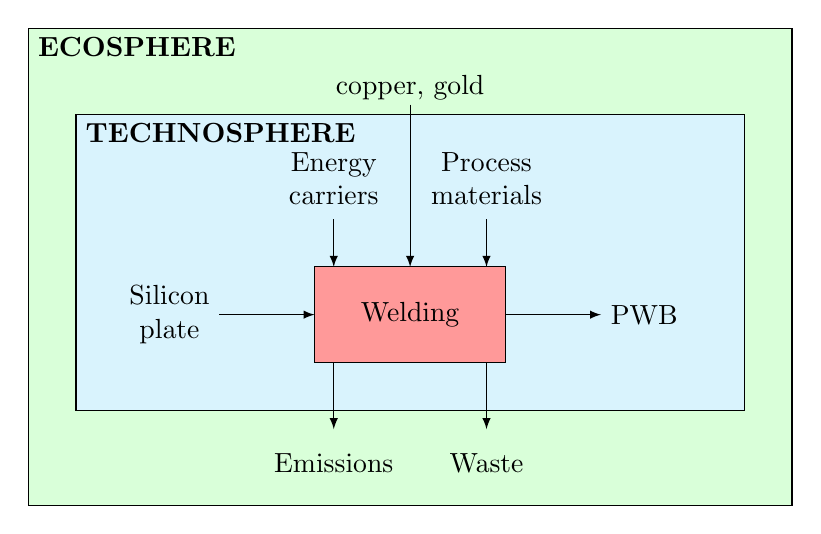
\begin{tikzpicture}[every text node part/.style={align=center}]
        \draw[fill=green!15, draw=black] (0, 0) rectangle (0.8\textwidth, 0.5\textwidth);
        \draw[fill=cyan!15, draw=black] (0.05\textwidth, 0.1\textwidth) rectangle (0.75\textwidth, 0.41\textwidth);

        \node(Ecosphere) at (0, 0.5\textwidth)[anchor=north west]{\textbf{ECOSPHERE}};
        \node(Technosphere) at (0.05\textwidth, 0.41\textwidth)[anchor=north west]{\textbf{TECHNOSPHERE}};

        \draw[fill=red!40, draw=black] (0.3\textwidth,0.15\textwidth) rectangle (0.5\textwidth,0.25\textwidth);
        \node(process) at (0.4\textwidth, 0.2\textwidth)[anchor=center]{Welding};

        \draw[->, >=latex](0.4\textwidth, 0.42\textwidth) -- node[anchor=south, yshift=0.08\textwidth]{copper, gold}(0.4\textwidth, 0.25\textwidth);
        \draw[->, >=latex](0.2\textwidth, 0.2\textwidth) -- node[anchor=east, xshift=-0.05\textwidth]{Silicon\\plate}(0.3\textwidth, 0.2\textwidth);
        \draw[->, >=latex](0.5\textwidth, 0.2\textwidth) -- node[anchor=west, xshift=0.05\textwidth]{PWB}(0.6\textwidth, 0.2\textwidth);
        \draw[->, >=latex](0.48\textwidth, 0.15\textwidth) -- node[anchor=north, yshift=-0.05\textwidth]{Waste}(0.48\textwidth, 0.08\textwidth);
        \draw[->, >=latex](0.32\textwidth, 0.15\textwidth) -- node[anchor=north, yshift=-0.05\textwidth]{Emissions}(0.32\textwidth, 0.08\textwidth);
        \draw[->, >=latex](0.32\textwidth, 0.3\textwidth) -- node[anchor=south, yshift=0.03\textwidth]{Energy\\carriers}(0.32\textwidth, 0.25\textwidth);
        \draw[->, >=latex](0.48\textwidth, 0.3\textwidth) -- node[anchor=south, yshift=0.03\textwidth]{Process\\materials}(0.48\textwidth, 0.25\textwidth);
        
    \end{tikzpicture}
    \caption{Example for an eco- and technosphere analysis for an individual process for the digital note-taking scenario.}\label{fig:eco_technosphere_digital}
\end{figure}

Following this distinction, all pieces of data must be classified as being foreground or background data. For this investigation, this step is facilitated by the use of the EcoInvent database within the \textsc{SimaPro} software. Most of the processes described for each investigation will be taken as background data since their information is widely available in the EcoInvent database and only the top-level assembly definitions are taken as foreground data since they must be explicitly given. A through description for these (sub)assemblies is given in the following section for both note-taking scenarios.

Finally, the system boundaries must be clearly stated. This is a crucial step since it can determine the outcome of an investigation, specifically when comparing multiple test cases. For this investigation, only the materials, processes, transportation and energy required for the manufacturing, use and disposal of both test cases is considered over a period of five academic years. Impacts caused by the manufacturing of the machines involved in the industrial and transportation processes of the material for the investigated test cases are not included.